% !TEX root = ../main.tex
\section{Dust Kin} \label{kin::oth}
\DndDropCapLine{T}{he light beckons, and you follow.}
\textit{As the light lead you once, now you are guided by enlightenment.
With each hidden truth you uncover, you learn more of what the world is, and how to secure your place in it.
Secrets are your power and your currency.
Seek them out, and guard them well.}

\hspace*{\fill} --- Ancient Moonborn saying.

Moody and perplexing.
Isolated and elegant.
Tough and passionate.
The ways in which one might describe the dust kin are many.
The dust kin, oths, or szua-tlekeloo rlue are a quiet species with a tendency towards nature and knowledge.
They're a solitary yet intimate creature with a penchant for nature and ritual.

\subsection*{Enigmatic and Uncanny}
    While oths can be see as much as gats or irds around civilized lands, they are far more mysterious and reclusive than the two.
    Often silent, oths have a reputation for being cryptic and thoughtful.
    They tend to follow their intuition on a whim.

    Oths usually travel with a large scroll in their backs made from their own fabric, which they protect with impermeable and resilient guards.
    This scroll is a compendium of knowledge passed down through generations, and they add to it in key moments in their life.

    The dust kin have large, heavy forewings that hang around their humanoid bodies like cloaks, which hide a shorter and more delicate set of hindwings behind them.
    They have two sets of arms, one above the other.
    The upper pair is strong and long, while the lower one is weak, and mostly left for secondary tasks.
    Their feet have three fingers and their arms have four, with one being an opposable thumb.
    They have an insectoid face with antennae and compound eyes.
    Their body is covered in a short, fluffy hair which is usually of a very pale brown color.

\subsection*{Long Tempers}
    Through generational learning, oths are wise and prudent creatures from a very early age.
    Many chase intellectual or mindful pursuits, becoming librarians and philosophers.
    They pontificate on the nature of life and knowledge.
    Most think that the oth are naturally intelligent, and take their opinions with very high regard.

    While most dedicate to cultivating their cognition, some decide to live their lives in adventure.
    They nurture their minds with experience, acquiring knowledge via facing the challenges of the world.

    A common thread throughout the race is that they are slow to anger.
    Regardless of culture, it is instilled in them as early as the larval stage.
    Life is too short to be spent in anger or frustration.

\subsection*{Cycle of Resurrection}
    An oth knows when their natural death approaches, and faces it peacefully.
    When they are near their death, they say their goodbyes and withdraws from civilized society.
    The oth then pilgrimages towards a cavern or secret place they designated during their lifetime.

    On arrival, the oth blocks all but one entrance to this sacred place, and lays ten to twenty eggs in a bed of silk during fall.
    They then spend their time gathering foodstuffs and lining the walls, floor, and roof with silk, providing a safe environment for their descendants to develop in.
    The oth also uses this time to finish writing their compendium of knowledge in their scroll, developing it until its ready to be passed on to their strongest descendant.

    At the last week before the break of summer, the oth closes the last entrance to its sacred place, engulfing it in total darkness.
    And they wait.

    At some point during summer, the eggs hatch for their parent to greet and nourish their newborn larvae.
    They dying oth hands qualars to their progeny, teaching them their language and the way of the world.
    Along with this they pass on the tenets of their culture.
    The parent eats no more than a grain of rice per day, and refrains almost completely from liquids.

    Six months after hatching, the younglings go through the process of pupation, remaining as pupa for a year.
    The parent uses this time to drink an embalming fluid, and mummifies themselves in silk.
    They slowly lose their sentience, peacefully drifting into non-existence.

    After hatching, the oths pay tribute to their now dead parent, and re-seal their cradle.
    The first place they see becomes their parent's final resting place.
    The oths then travel together, forming a small familiar tribe which lasts until they reach maturity.
    While the members of the family may part ways, the bond they share is never truly broken.

\subsection*{Educated by Experience}
    Due to the way the oths spend their youths, they are generally very wise from a very young age, blessed with the knowledge of the previous generations.
    However, it's in an oth's nature to cultivate this wisdom with a contemporary and personal viewpoint of the world.
    It's rare to see an oth not spending much of their youth travelling for knowledge and wisdom.
    % The dust kin is also very concerned about the preservation of nature, and are experts at recording its sights and dwellers in great detail.

\subsection*{Oth Names}
    In oth culture, the parent is assigned the task of naming each of their children in their larval stage.
    These names will often change at the whim of the parent, not becoming official until pupation.
    Their names are often difficult to pronounce by the other kins, and most don't mind being called by a nickname for simplicity.
    The dust kin doesn't use family names, recognizing their relatives by sight alone.

    \paragraph{Names}
    Adz'kt, Andle, Axa, Bixi, Chch, Chith, Daph, Fen'kt, Fl'ka, Fra, G'zigg, Gl'rik, Hadae, Iitus, J'llkx, Kl'il, Lenna, L'kpha, Mlf, N'kakt, Riz, Scelkt, Sud'kx, Thm, Timpth, Zkx.

% \begin{table*}[b]%
%     \begin{DndTable}[width=\linewidth, header=Oth Silk Armor]{lXXXX}
%         \textbf{Armor} & \textbf{AC} & \textbf{DC} & \textbf{Time taken} & \textbf{Cost} \\
%         Silk Armor                & 11 + Dex mod     & 10 & 1 week   &    -    \\
%         Reinforced Silk Armor     & 12 + Dex mod     & 15 & 2 weeks  &   10 GP \\
%         Exquisite Silk Armor (+1) & 12 + Dex mod + 1 & 20 & 1 month  &  100 GP \\
%         Excellent Silk Armor (+2) & 12 + Dex mod + 2 & 20 & 6 months & 1000 GP
%     \end{DndTable}
% \end{table*}

\subsection*{Traits}
    Your oth character has the following set of skills, based on its customs and ancestry.

    \subparagraph{Ability Score Increase} Your Intelligence score increases by 2.

    \subparagraph{Age} An oth will go through three stages of growth: eggs, larvae, and pupa.
    This development takes in total about two years.
    In terms of maturity, they emerge from their pupa as adults, but reach full size at about ten years of age.
    Oths live to be around 80 years old.

    \subparagraph{Alignment} Oth tend to stray from extremes, most often remaining neutral in conflicts as long as there is no direct danger to themselves or those close to them.
    The oths passion for wisdom leads them to the blue tide.

    \subparagraph{Size} Oth typically range from between 135 to just under 180 cm.
    Your size if Medium.
    You are impressively lightweight for your size, weighing around 45 kg.

    \subparagraph{Speed} Your base walking speed it 9 meters.

    \subparagraph{Clumsy Flight} Once per short rest, you can fly with a speed of 6 meters for a number of rounds equal to your Constitution modifier plus 2, with a minimum of 2 rounds.
    You cannot use this feature while you wear heavy armor or carry heavy weapons.

    \subparagraph{Darkvision} Due to your nocturnal heritage you have a good sense of vision in the dark.
    You can see in dim light within 18 meters of you as if it were bright light, and in darkness as if it were dim light.
    You can't discern color in darkness, only shades of gray.

\begin{figure}[!t]
    \centering
    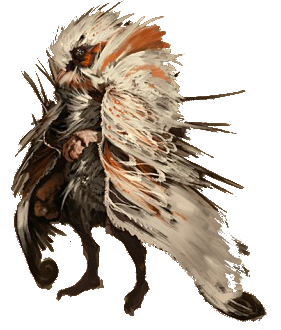
\includegraphics[width=0.48\textwidth]{04kins/img/14oth_white.png}
\end{figure}

    \subparagraph{Four-armed} You have a pair of weaker secondary arms that can be used to hold small objects and perform simple tasks.
    You cannot use these arms to wield weapons or shields and Strength checks using them are made with disadvantage.
    Due to your unique form, armor may need to be specially made, leading to additional costs.

    \subparagraph{Languages} You know how to speak, read, and write Shamabic and one other language of your choice.

\subsubsection{Moonborn}
    The moonborn are the most common of the oth.
    They prefer shady areas, and tend to live their lives in such places.
    They have been properly schooled under the light of Nuagal as oth tradition dictates, and many can be found in darkened libraries during daytime.

    As their name suggests, moonborn have a special affinity for Nuagal, and can even feed off its light.
    They travel at night and hide during the day, and most carry a specially designed tent that blocks all incoming sunlight.

    \subparagraph{Ability Score Increase} Your Wisdom score is increased by 1.

    \subparagraph{Light Sensitivity} Moonborn grow away from the sun.
    You are vulnerable against radiant damage.
    You have disadvantage on attack rolls and Wisdom (Perception) checks that rely on sight when you, the target of your attack, or what you are trying to perceive is under direct sunlight.

    \subparagraph{Sensitive Antennae} Using your specialized antennae, you have advantage on perception checks that rely on smell.

    \subparagraph{Lunar Studies} You are competent in the Religion and History skills.

    \subparagraph{Moon Magic} You know the Light cantrip (page \pageref{spell::light}).
    When you gain your third hit die, you learn the Faerie Fire spell (page \pageref{spell::faeriefire}), which you can cast once per day.
    When you get your fifth hit die, you learn the Glitterdust spell (page \pageref{spell::glitterdust}), which you can cast once per day.

    Intelligence is your spellcasting modifier for these spells.

\subsubsection{Chu'ash Kin}
    The chu'ash oths are a subculture that differentiate from the rest by their curious and reckless nature.
    Weaker than their siblings, they are born a summer too late, and never get to meet their parent.
    They are instead cared for by their older siblings, and are the younger members of their familiar tribes.

    To most, a chu'ash oth seems perpetually disorganized and distracted, which leads to the belief that they have a lower intelligence to the other of their kin.
    In truth, the chu'ash have a unique perception of the world.
    They are able to interpret information in a unique way, allowing them to see possibilities other cannot.
    Born with an untamed intelligence, the chu'ash oth has an affinity to find the hidden patterns of the world.

    \subparagraph{Ability Score Increase} Your Charisma score is increased by 1.

    \subparagraph{Fated} Whether luck of a guiding presence, you always seem to find your way.
    Once per day you can choose to reroll an attack, skill check, or saving throw.
    You can decide to do this after the roll, but before the outcome of the roll has been determined.

    \subparagraph{Touched} You know the Dancing Lights cantrip (page \pageref{spell::dancinglights}).
    When you gain your third hit die, you learn the Color Spray spell (page \pageref{spell::colorspray}), which you can cast once per day.
    When you get your fifth hit die, you learn the Blur spell (page \pageref{spell::blur}), which you can cast once per day.

    Charisma is your spellcasting modifier for these spells.

\subsubsection{Sunstruck Oth}
    While most oths follow the circle of resurrection to the letter, there are a few who choose to ignore it.
    They lay their eggs under direct sunlight, and their larvae quickly lose their fragile hindwings.
    Unrepairable, their wings stay atrophied and shriveled thorough their lives.

    These oths are known as the sunstruck, and they've earn a reputation of unpaired hardiness and resilience.
    The clans of Shief and Zmiva cherish this attribute, and consciously molt in lit areas to engender it.

    \subparagraph{Ability Score Increase} Due to your hardiness, your Constitution score is increased by 1.

    \subparagraph{Sunstruck Birth} You lose your \textbf{Clumsy Flight} and \textbf{Darkvision} traits.

    \subparagraph{Photosynthesis} While you need water like any other creature, you don't need to eat to gain sustenance.
    You can choose to instead collect light with your wings via photosynthesis.
    Each day, you must spend two hours with your hindwings exposed to sunlight, or four hours to moonlight to be properly well fed.

    \subparagraph{Sunstruck Resilience} You are competent in the Survival skill.

    \subparagraph{Vertical Takeoff} As an action, you can use your powerful frame and knowledge of thermals to propel yourself upward a distance equal to double your movement speed.
    This technique is used by the Shief scouts to survey the desert around them in search of food or predators.

    \subparagraph{Slow Fall} While useless for flight, your shriveled wings allow you to slow your fall.
    When falling, you can use an action or reaction to lift your wings using your second pair of arms to slow your descent.
    You continue to fall gently at a speed of 9 meters per round, taking no fall damage when you land.
    You cannot use this trait if you are wearing heavy armor or are encumbered.

\newpage
